\documentclass{beamer} 
\usetheme{uniud}
\usepackage{xspace}
\usepackage{graphicx}
\usepackage{verbatim}
\usepackage{FCNCsupport-defs}
\usepackage{FCNCpaths}
\usepackage{multirow}
\setlength{\textwidth}{11cm}
\setlength{\textheight}{6cm} 
\usepackage{geometry}
\geometry{papersize={14.5cm,11cm}} 

\title{Status report}
\date{\today}
\author[Boyang Li]{
  Boyang Li \\
}

\begin{document}

\begin{frame}
\titlepage
\end{frame}

\section{Updated yield table}
\begin{tiny} 
\begin{table}
\footnotesize
\caption{The sample and data yield before the fit.}
\centering
\begin{tabular}{|c|c|c|c|c|} \hline
 & $l\thadhad$ ss & $l\thadhad$ os & STH $\tlhad$ ss & STH $\tlhad$ os\\\hline
data & $24.00\pm4.90$ & $28.00\pm5.29$ & $468.00\pm21.63$ & $6787.00\pm82.38$\\\hline
background & $28.34\pm1.91$ & $22.52\pm1.73$ & $459.96\pm8.96$ & $7004.75\pm32.28$\\\hline
$\bar{t}t\to bWcH$ & $0.29\pm0.04$ & $7.13\pm0.21$ & $7.05\pm0.20$ & $12.49\pm0.32$\\\hline
$cg\to tH$ & $0.01\pm0.00$ & $0.14\pm0.01$ & $0.15\pm0.01$ & $0.40\pm0.02$\\\hline
tcH~merged~signal & $0.30\pm0.04$ & $7.27\pm0.21$ & $7.20\pm0.20$ & $12.89\pm0.32$\\\hline
$\bar{t}t\to bWuH$ & $0.10\pm0.03$ & $0.84\pm0.07$ & $2.37\pm0.12$ & $3.92\pm0.17$\\\hline
$ug\to tH$ & $0.01\pm0.01$ & $0.23\pm0.03$ & $0.79\pm0.05$ & $1.79\pm0.09$\\\hline
tuH~merged~signal & $0.12\pm0.03$ & $1.07\pm0.08$ & $3.16\pm0.13$ & $5.72\pm0.20$\\\hline
\end{tabular}
\begin{tabular}{|c|c|c|c|c|} \hline
 & TTH $\tlhad$ ss & TTH $\tlhad$ os & $l\thadhad$ 2b ss & $l\thadhad$ 2b os\\\hline
data & $556.00\pm23.58$ & $4147.00\pm64.40$ & $75.00\pm8.66$ & $92.00\pm9.59$\\\hline
background & $511.26\pm9.76$ & $4342.91\pm24.01$ & $89.79\pm3.36$ & $79.48\pm3.09$\\\hline
$\bar{t}t\to bWcH$ & $4.61\pm0.17$ & $14.86\pm0.38$ & $0.22\pm0.04$ & $4.17\pm0.16$\\\hline
$cg\to tH$ & $0.06\pm0.01$ & $0.25\pm0.02$ & $0.00\pm0.00$ & $0.09\pm0.01$\\\hline
tcH~merged~signal & $4.68\pm0.17$ & $15.11\pm0.38$ & $0.23\pm0.04$ & $4.26\pm0.16$\\\hline
$\bar{t}t\to bWuH$ & $1.94\pm0.11$ & $3.97\pm0.18$ & $0.04\pm0.02$ & $0.44\pm0.05$\\\hline
$ug\to tH$ & $0.28\pm0.04$ & $1.11\pm0.08$ & $0.00\pm0.01$ & $0.23\pm0.03$\\\hline
tuH~merged~signal & $2.22\pm0.11$ & $5.08\pm0.20$ & $0.04\pm0.02$ & $0.67\pm0.06$\\\hline
\end{tabular}
\begin{tabular}{|c|c|c|c|c|} \hline
 & STH $\tlhad$ 2b ss & STH $\tlhad$ 2b os & TTH $\tlhad$ 2b ss & TTH $\tlhad$ 2b os\\\hline
data & $739.00\pm27.18$ & $9247.00\pm96.16$ & $622.00\pm24.94$ & $4689.00\pm68.48$\\\hline
background & $815.62\pm10.25$ & $9649.40\pm35.13$ & $575.99\pm8.45$ & $4865.38\pm24.75$\\\hline
$\bar{t}t\to bWcH$ & $1.88\pm0.10$ & $5.36\pm0.23$ & $1.21\pm0.08$ & $4.30\pm0.21$\\\hline
$cg\to tH$ & $0.02\pm0.00$ & $0.12\pm0.01$ & $0.02\pm0.00$ & $0.04\pm0.01$\\\hline
tcH~merged~signal & $1.90\pm0.10$ & $5.47\pm0.23$ & $1.23\pm0.08$ & $4.34\pm0.21$\\\hline
$\bar{t}t\to bWuH$ & $0.70\pm0.06$ & $1.28\pm0.10$ & $0.36\pm0.05$ & $1.09\pm0.10$\\\hline
$ug\to tH$ & $0.12\pm0.02$ & $0.50\pm0.05$ & $0.06\pm0.01$ & $0.27\pm0.04$\\\hline
tuH~merged~signal & $0.81\pm0.07$ & $1.78\pm0.11$ & $0.43\pm0.05$ & $1.36\pm0.10$\\\hline
\end{tabular}
\label{tab:yield}
\end{table}

\end{tiny} 
\newpage
\frame{
\begin{footnotesize} 
\begin{table}
\footnotesize
\caption{The sample and data yield before the fit.}
\centering
\begin{tabular}{|c|c|c|c|c|} \hline
 & $l\thadhad$ ss & $l\thadhad$ os & STH $\tlhad$ ss & STH $\tlhad$ os\\\hline
data & $24.00\pm4.90$ & $28.00\pm5.29$ & $468.00\pm21.63$ & $6787.00\pm82.38$\\\hline
background & $28.34\pm1.91$ & $22.52\pm1.73$ & $459.96\pm8.96$ & $7004.75\pm32.28$\\\hline
$\bar{t}t\to bWcH$ & $0.29\pm0.04$ & $7.13\pm0.21$ & $7.05\pm0.20$ & $12.49\pm0.32$\\\hline
$cg\to tH$ & $0.01\pm0.00$ & $0.14\pm0.01$ & $0.15\pm0.01$ & $0.40\pm0.02$\\\hline
tcH~merged~signal & $0.30\pm0.04$ & $7.27\pm0.21$ & $7.20\pm0.20$ & $12.89\pm0.32$\\\hline
$\bar{t}t\to bWuH$ & $0.10\pm0.03$ & $0.84\pm0.07$ & $2.37\pm0.12$ & $3.92\pm0.17$\\\hline
$ug\to tH$ & $0.01\pm0.01$ & $0.23\pm0.03$ & $0.79\pm0.05$ & $1.79\pm0.09$\\\hline
tuH~merged~signal & $0.12\pm0.03$ & $1.07\pm0.08$ & $3.16\pm0.13$ & $5.72\pm0.20$\\\hline
\end{tabular}
\begin{tabular}{|c|c|c|c|c|} \hline
 & TTH $\tlhad$ ss & TTH $\tlhad$ os & $l\thadhad$ 2b ss & $l\thadhad$ 2b os\\\hline
data & $556.00\pm23.58$ & $4147.00\pm64.40$ & $75.00\pm8.66$ & $92.00\pm9.59$\\\hline
background & $511.26\pm9.76$ & $4342.91\pm24.01$ & $89.79\pm3.36$ & $79.48\pm3.09$\\\hline
$\bar{t}t\to bWcH$ & $4.61\pm0.17$ & $14.86\pm0.38$ & $0.22\pm0.04$ & $4.17\pm0.16$\\\hline
$cg\to tH$ & $0.06\pm0.01$ & $0.25\pm0.02$ & $0.00\pm0.00$ & $0.09\pm0.01$\\\hline
tcH~merged~signal & $4.68\pm0.17$ & $15.11\pm0.38$ & $0.23\pm0.04$ & $4.26\pm0.16$\\\hline
$\bar{t}t\to bWuH$ & $1.94\pm0.11$ & $3.97\pm0.18$ & $0.04\pm0.02$ & $0.44\pm0.05$\\\hline
$ug\to tH$ & $0.28\pm0.04$ & $1.11\pm0.08$ & $0.00\pm0.01$ & $0.23\pm0.03$\\\hline
tuH~merged~signal & $2.22\pm0.11$ & $5.08\pm0.20$ & $0.04\pm0.02$ & $0.67\pm0.06$\\\hline
\end{tabular}
\begin{tabular}{|c|c|c|c|c|} \hline
 & STH $\tlhad$ 2b ss & STH $\tlhad$ 2b os & TTH $\tlhad$ 2b ss & TTH $\tlhad$ 2b os\\\hline
data & $739.00\pm27.18$ & $9247.00\pm96.16$ & $622.00\pm24.94$ & $4689.00\pm68.48$\\\hline
background & $815.62\pm10.25$ & $9649.40\pm35.13$ & $575.99\pm8.45$ & $4865.38\pm24.75$\\\hline
$\bar{t}t\to bWcH$ & $1.88\pm0.10$ & $5.36\pm0.23$ & $1.21\pm0.08$ & $4.30\pm0.21$\\\hline
$cg\to tH$ & $0.02\pm0.00$ & $0.12\pm0.01$ & $0.02\pm0.00$ & $0.04\pm0.01$\\\hline
tcH~merged~signal & $1.90\pm0.10$ & $5.47\pm0.23$ & $1.23\pm0.08$ & $4.34\pm0.21$\\\hline
$\bar{t}t\to bWuH$ & $0.70\pm0.06$ & $1.28\pm0.10$ & $0.36\pm0.05$ & $1.09\pm0.10$\\\hline
$ug\to tH$ & $0.12\pm0.02$ & $0.50\pm0.05$ & $0.06\pm0.01$ & $0.27\pm0.04$\\\hline
tuH~merged~signal & $0.81\pm0.07$ & $1.78\pm0.11$ & $0.43\pm0.05$ & $1.36\pm0.10$\\\hline
\end{tabular}
\label{tab:yield}
\end{table}

\end{footnotesize} 
}
\newpage
\section{Updated BDT training}

\input{\FCNCFigures/tex/BDT}
\begin{tiny} 
\input{\FCNCTables/tthML/Importance}
\end{tiny} 
\newpage
\section{Updated significance table}
\begin{tiny} 
\centering
\begin{tabular}{|c|c|c|c|c|} \hline
 & 1l1tau1b1j ss e  highmet & 1l1tau1b1j ss e  lowmet & 1l1tau1b1j ss mu  highmet & 1l1tau1b1j ss mu  lowmet\\\hline
$\bar{t}t\to bWcH$ & $0.61$ & $0.23$ & $1.11$ & $0.34$\\\hline
$cg\to tH$ & $0.02$ & $0.01$ & $0.04$ & $0.01$\\\hline
tcH~merged~signal & $0.63$ & $0.24$ & $1.15$ & $0.35$\\\hline
$\bar{t}t\to bWuH$ & $0.64$ & $0.22$ & $1.18$ & $0.39$\\\hline
$ug\to tH$ & $0.05$ & $0.02$ & $0.28$ & $0.09$\\\hline
tuH~merged~signal & $0.70$ & $0.24$ & $1.45$ & $0.48$\\\hline
\end{tabular}
\begin{tabular}{|c|c|c|c|c|} \hline
 & 1l1tau1b2j os e  highmet & 1l1tau1b2j os e  lowmet & 1l1tau1b2j os mu  highmet & 1l1tau1b2j os mu  lowmet\\\hline
$\bar{t}t\to bWcH$ & $0.35$ & $0.13$ & $0.57$ & $0.25$\\\hline
$cg\to tH$ & $0.04$ & $0.01$ & $0.05$ & $0.01$\\\hline
tcH~merged~signal & $0.38$ & $0.14$ & $0.62$ & $0.27$\\\hline
$\bar{t}t\to bWuH$ & $0.36$ & $0.15$ & $0.60$ & $0.23$\\\hline
$ug\to tH$ & $0.21$ & $0.04$ & $0.35$ & $0.07$\\\hline
tuH~merged~signal & $0.55$ & $0.19$ & $0.92$ & $0.30$\\\hline
\end{tabular}
\begin{tabular}{|c|c|c|c|c|} \hline
 & 1l1tau1b2j ss e  highmet & 1l1tau1b2j ss e  lowmet & 1l1tau1b2j ss mu  highmet & 1l1tau1b2j ss mu  lowmet\\\hline
$\bar{t}t\to bWcH$ & $0.59$ & $0.19$ & $1.07$ & $0.35$\\\hline
$cg\to tH$ & $0.02$ & $0.00$ & $0.03$ & $0.01$\\\hline
tcH~merged~signal & $0.61$ & $0.20$ & $1.10$ & $0.36$\\\hline
$\bar{t}t\to bWuH$ & $0.64$ & $0.23$ & $1.13$ & $0.43$\\\hline
$ug\to tH$ & $0.03$ & $0.01$ & $0.23$ & $0.08$\\\hline
tuH~merged~signal & $0.68$ & $0.24$ & $1.35$ & $0.51$\\\hline
\end{tabular}
\begin{tabular}{|c|c|c|c|c|} \hline
 & 1l1tau1b3j os e  highmet & 1l1tau1b3j os e  lowmet & 1l1tau1b3j os mu  highmet & 1l1tau1b3j os mu  lowmet\\\hline
$\bar{t}t\to bWcH$ & $0.76$ & $0.28$ & $1.18$ & $0.50$\\\hline
$cg\to tH$ & $0.04$ & $0.01$ & $0.05$ & $0.02$\\\hline
tcH~merged~signal & $0.79$ & $0.29$ & $1.23$ & $0.51$\\\hline
$\bar{t}t\to bWuH$ & $0.77$ & $0.34$ & $1.28$ & $0.51$\\\hline
$ug\to tH$ & $0.22$ & $0.04$ & $0.30$ & $0.08$\\\hline
tuH~merged~signal & $0.98$ & $0.38$ & $1.58$ & $0.59$\\\hline
\end{tabular}
\begin{tabular}{|c|c|c|c|c|} \hline
 & 1l1tau1b3j ss e  highmet & 1l1tau1b3j ss e  lowmet & 1l1tau1b3j ss mu  highmet & 1l1tau1b3j ss mu  lowmet\\\hline
$\bar{t}t\to bWcH$ & $0.29$ & $0.09$ & $0.48$ & $0.16$\\\hline
$cg\to tH$ & $0.01$ & $0.00$ & $0.01$ & $0.00$\\\hline
tcH~merged~signal & $0.30$ & $0.09$ & $0.49$ & $0.17$\\\hline
$\bar{t}t\to bWuH$ & $0.31$ & $0.10$ & $0.54$ & $0.18$\\\hline
$ug\to tH$ & $0.03$ & $0.01$ & $0.06$ & $0.02$\\\hline
tuH~merged~signal & $0.33$ & $0.11$ & $0.60$ & $0.20$\\\hline
\end{tabular}
\begin{tabular}{|c|c|c|c|c|} \hline
 & 1l1tau2b1j ss e  highmet & 1l1tau2b1j ss e  lowmet & 1l1tau2b1j ss mu  highmet & 1l1tau2b1j ss mu  lowmet\\\hline
$\bar{t}t\to bWcH$ & $0.12$ & $0.07$ & $0.20$ & $0.06$\\\hline
$cg\to tH$ & $0.00$ & $0.00$ & $0.00$ & $0.00$\\\hline
tcH~merged~signal & $0.12$ & $0.07$ & $0.21$ & $0.06$\\\hline
$\bar{t}t\to bWuH$ & $0.04$ & $0.01$ & $0.08$ & $0.02$\\\hline
$ug\to tH$ & $0.01$ & $0.00$ & $0.02$ & $0.01$\\\hline
tuH~merged~signal & $0.04$ & $0.01$ & $0.10$ & $0.03$\\\hline
\end{tabular}
\begin{tabular}{|c|c|c|c|c|} \hline
 & 1l1tau2b2j os e  highmet & 1l1tau2b2j os e  lowmet & 1l1tau2b2j os mu  highmet & 1l1tau2b2j os mu  lowmet\\\hline
$\bar{t}t\to bWcH$ & $0.10$ & $0.03$ & $0.14$ & $0.07$\\\hline
$cg\to tH$ & $0.00$ & $0.00$ & $0.01$ & $0.00$\\\hline
tcH~merged~signal & $0.10$ & $0.03$ & $0.15$ & $0.07$\\\hline
$\bar{t}t\to bWuH$ & $0.03$ & $0.02$ & $0.07$ & $0.02$\\\hline
$ug\to tH$ & $0.02$ & $0.02$ & $0.03$ & $0.01$\\\hline
tuH~merged~signal & $0.04$ & $0.03$ & $0.10$ & $0.03$\\\hline
\end{tabular}
\begin{tabular}{|c|c|c|c|c|} \hline
 & 1l1tau2b2j ss e  highmet & 1l1tau2b2j ss e  lowmet & 1l1tau2b2j ss mu  highmet & 1l1tau2b2j ss mu  lowmet\\\hline
$\bar{t}t\to bWcH$ & $0.07$ & $0.06$ & $0.14$ & $0.04$\\\hline
$cg\to tH$ & $0.00$ & $0.00$ & $0.00$ & $0.00$\\\hline
tcH~merged~signal & $0.07$ & $0.06$ & $0.14$ & $0.04$\\\hline
$\bar{t}t\to bWuH$ & $0.04$ & $0.01$ & $0.07$ & $0.02$\\\hline
$ug\to tH$ & $0.00$ & $0.00$ & $0.02$ & $0.01$\\\hline
tuH~merged~signal & $0.05$ & $0.01$ & $0.08$ & $0.03$\\\hline
\end{tabular}
\begin{tabular}{|c|c|c|c|c|} \hline
 & 1l1tau2b3j os e  highmet & 1l1tau2b3j os e  lowmet & 1l1tau2b3j os mu  highmet & 1l1tau2b3j os mu  lowmet\\\hline
$\bar{t}t\to bWcH$ & $0.14$ & $0.03$ & $0.20$ & $0.10$\\\hline
$cg\to tH$ & $0.00$ & $0.00$ & $0.00$ & $0.00$\\\hline
tcH~merged~signal & $0.14$ & $0.03$ & $0.21$ & $0.10$\\\hline
$\bar{t}t\to bWuH$ & $0.07$ & $0.03$ & $0.10$ & $0.04$\\\hline
$ug\to tH$ & $0.01$ & $0.00$ & $0.03$ & $0.01$\\\hline
tuH~merged~signal & $0.08$ & $0.03$ & $0.13$ & $0.04$\\\hline
\end{tabular}
\begin{tabular}{|c|c|c|c|c|} \hline
 & 1l1tau2b3j ss e  highmet & 1l1tau2b3j ss e  lowmet & 1l1tau2b3j ss mu  highmet & 1l1tau2b3j ss mu  lowmet\\\hline
$\bar{t}t\to bWcH$ & $0.04$ & $0.01$ & $0.08$ & $0.02$\\\hline
$cg\to tH$ & $0.00$ & $0.00$ & $0.00$ & $0.00$\\\hline
tcH~merged~signal & $0.04$ & $0.01$ & $0.08$ & $0.02$\\\hline
$\bar{t}t\to bWuH$ & $0.03$ &  / & $0.04$ & $0.02$\\\hline
$ug\to tH$ & $0.00$ &  / & $0.01$ & $0.00$\\\hline
tuH~merged~signal & $0.03$ &  / & $0.04$ & $0.02$\\\hline
\end{tabular}
\begin{tabular}{|c|c|c|c|c|} \hline
 & 1l2tau1bnj os e  highmet & 1l2tau1bnj os e  lowmet & 1l2tau1bnj os mu  highmet & 1l2tau1bnj os mu  lowmet\\\hline
$\bar{t}t\to bWcH$ & $3.27$ & $1.47$ & $4.80$ & $2.71$\\\hline
$cg\to tH$ & $0.37$ & $0.12$ & $0.47$ & $0.26$\\\hline
tcH~merged~signal & $3.47$ & $1.55$ & $5.13$ & $2.88$\\\hline
$\bar{t}t\to bWuH$ & $3.55$ & $1.67$ & $5.04$ & $2.89$\\\hline
$ug\to tH$ & $0.65$ & $0.27$ & $2.30$ & $1.28$\\\hline
tuH~merged~signal & $3.92$ & $1.86$ & $6.76$ & $3.80$\\\hline
\end{tabular}
\begin{tabular}{|c|c|c|c|c|} \hline
 & 1l2tau1bnj ss e  highmet & 1l2tau1bnj ss e  lowmet & 1l2tau1bnj ss mu  highmet & 1l2tau1bnj ss mu  lowmet\\\hline
$\bar{t}t\to bWcH$ & $0.13$ & $0.15$ & $0.22$ & $0.14$\\\hline
$cg\to tH$ & $0.01$ & $0.01$ & $0.01$ & $0.01$\\\hline
tcH~merged~signal & $0.14$ & $0.16$ & $0.23$ & $0.14$\\\hline
$\bar{t}t\to bWuH$ & $0.18$ & $0.15$ & $0.24$ & $0.18$\\\hline
$ug\to tH$ & $0.05$ & $0.05$ & $0.07$ & $0.04$\\\hline
tuH~merged~signal & $0.22$ & $0.18$ & $0.31$ & $0.21$\\\hline
\end{tabular}
\begin{tabular}{|c|c|c|c|c|} \hline
 & 1l2tau2bnj os e  highmet & 1l2tau2bnj os e  lowmet & 1l2tau2bnj os mu  highmet & 1l2tau2bnj os mu  lowmet\\\hline
$\bar{t}t\to bWcH$ & $0.50$ & $0.60$ & $0.73$ & $0.38$\\\hline
$cg\to tH$ & $0.01$ & $0.02$ & $0.02$ & $0.01$\\\hline
tcH~merged~signal & $0.51$ & $0.61$ & $0.75$ & $0.39$\\\hline
$\bar{t}t\to bWuH$ & $0.15$ & $0.04$ & $0.18$ & $0.10$\\\hline
$ug\to tH$ & $0.01$ & $0.01$ & $0.07$ & $0.02$\\\hline
tuH~merged~signal & $0.16$ & $0.04$ & $0.25$ & $0.12$\\\hline
\end{tabular}
\begin{tabular}{|c|c|c|c|c|} \hline
 & 1l2tau2bnj ss e  highmet & 1l2tau2bnj ss mu  highmet & 1l2tau2bnj ss mu  lowmet & 1l1tau1b1j ss  highmet\\\hline
$\bar{t}t\to bWcH$ & $0.02$ & $0.03$ &  / & $1.26$\\\hline
$cg\to tH$ & $0.00$ & $0.01$ & $0.00$ & $0.05$\\\hline
tcH~merged~signal & $0.02$ & $0.03$ & $0.00$ & $1.31$\\\hline
$\bar{t}t\to bWuH$ & $0.01$ & $0.01$ &  / & $1.34$\\\hline
$ug\to tH$ &  / & $0.00$ &  / & $0.27$\\\hline
tuH~merged~signal & $0.01$ & $0.01$ &  / & $1.60$\\\hline
\end{tabular}
\begin{tabular}{|c|c|c|c|c|} \hline
 & 1l1tau1b1j ss  lowmet & 1l1tau1b2j os  highmet & 1l1tau1b2j os  lowmet & 1l1tau1b2j ss  highmet\\\hline
$\bar{t}t\to bWcH$ & $0.41$ & $0.67$ & $0.28$ & $1.22$\\\hline
$cg\to tH$ & $0.02$ & $0.06$ & $0.02$ & $0.03$\\\hline
tcH~merged~signal & $0.42$ & $0.73$ & $0.30$ & $1.26$\\\hline
$\bar{t}t\to bWuH$ & $0.45$ & $0.70$ & $0.28$ & $1.30$\\\hline
$ug\to tH$ & $0.09$ & $0.40$ & $0.08$ & $0.21$\\\hline
tuH~merged~signal & $0.53$ & $1.07$ & $0.35$ & $1.50$\\\hline
\end{tabular}
\begin{tabular}{|c|c|c|c|c|} \hline
 & 1l1tau1b2j ss  lowmet & 1l1tau1b3j os  highmet & 1l1tau1b3j os  lowmet & 1l1tau1b3j ss  highmet\\\hline
$\bar{t}t\to bWcH$ & $0.39$ & $1.40$ & $0.57$ & $0.56$\\\hline
$cg\to tH$ & $0.01$ & $0.06$ & $0.02$ & $0.01$\\\hline
tcH~merged~signal & $0.40$ & $1.46$ & $0.59$ & $0.57$\\\hline
$\bar{t}t\to bWuH$ & $0.48$ & $1.50$ & $0.61$ & $0.62$\\\hline
$ug\to tH$ & $0.07$ & $0.37$ & $0.09$ & $0.06$\\\hline
tuH~merged~signal & $0.55$ & $1.85$ & $0.70$ & $0.68$\\\hline
\end{tabular}
\begin{tabular}{|c|c|c|c|c|} \hline
 & 1l1tau1b3j ss  lowmet & 1l1tau2b1j ss  highmet & 1l1tau2b1j ss  lowmet & 1l1tau2b2j os  highmet\\\hline
$\bar{t}t\to bWcH$ & $0.19$ & $0.23$ & $0.08$ & $0.17$\\\hline
$cg\to tH$ & $0.00$ & $0.00$ & $0.00$ & $0.01$\\\hline
tcH~merged~signal & $0.19$ & $0.24$ & $0.08$ & $0.18$\\\hline
$\bar{t}t\to bWuH$ & $0.21$ & $0.09$ & $0.02$ & $0.07$\\\hline
$ug\to tH$ & $0.02$ & $0.02$ & $0.01$ & $0.04$\\\hline
tuH~merged~signal & $0.22$ & $0.11$ & $0.03$ & $0.11$\\\hline
\end{tabular}
\begin{tabular}{|c|c|c|c|c|} \hline
 & 1l1tau2b2j os  lowmet & 1l1tau2b2j ss  highmet & 1l1tau2b2j ss  lowmet & 1l1tau2b3j os  highmet\\\hline
$\bar{t}t\to bWcH$ & $0.07$ & $0.16$ & $0.06$ & $0.25$\\\hline
$cg\to tH$ & $0.00$ & $0.00$ & $0.00$ & $0.00$\\\hline
tcH~merged~signal & $0.07$ & $0.16$ & $0.06$ & $0.25$\\\hline
$\bar{t}t\to bWuH$ & $0.03$ & $0.08$ & $0.02$ & $0.13$\\\hline
$ug\to tH$ & $0.01$ & $0.02$ & $0.01$ & $0.03$\\\hline
tuH~merged~signal & $0.04$ & $0.09$ & $0.03$ & $0.15$\\\hline
\end{tabular}
\begin{tabular}{|c|c|c|c|c|} \hline
 & 1l1tau2b3j os  lowmet & 1l1tau2b3j ss  highmet & 1l1tau2b3j ss  lowmet & 1l2tau1bnj os  highmet\\\hline
$\bar{t}t\to bWcH$ & $0.10$ & $0.09$ & $0.02$ & $5.67$\\\hline
$cg\to tH$ & $0.00$ & $0.00$ & $0.00$ & $0.55$\\\hline
tcH~merged~signal & $0.10$ & $0.09$ & $0.02$ & $6.05$\\\hline
$\bar{t}t\to bWuH$ & $0.04$ & $0.05$ & $0.01$ & $6.01$\\\hline
$ug\to tH$ & $0.00$ & $0.01$ & $0.00$ & $2.33$\\\hline
tuH~merged~signal & $0.05$ & $0.05$ & $0.02$ & $7.71$\\\hline
\end{tabular}
\begin{tabular}{|c|c|c|c|c|} \hline
 & 1l2tau1bnj os  lowmet & 1l2tau1bnj ss  highmet & 1l2tau1bnj ss  lowmet & 1l2tau2bnj os  highmet\\\hline
$\bar{t}t\to bWcH$ & $3.00$ & $0.25$ & $0.19$ & $0.87$\\\hline
$cg\to tH$ & $0.27$ & $0.02$ & $0.01$ & $0.02$\\\hline
tcH~merged~signal & $3.19$ & $0.27$ & $0.19$ & $0.89$\\\hline
$\bar{t}t\to bWuH$ & $3.24$ & $0.29$ & $0.21$ & $0.22$\\\hline
$ug\to tH$ & $1.19$ & $0.09$ & $0.05$ & $0.06$\\\hline
tuH~merged~signal & $4.11$ & $0.37$ & $0.25$ & $0.29$\\\hline
\end{tabular}
\begin{tabular}{|c|c|c|c|c|} \hline
 & 1l2tau2bnj os  lowmet & 1l2tau2bnj ss  highmet & 1l2tau2bnj ss  lowmet & 1l1tau1b1j ss\\\hline
$\bar{t}t\to bWcH$ & $0.44$ & $0.03$ &  / & $1.33$\\\hline
$cg\to tH$ & $0.01$ & $0.00$ & $0.00$ & $0.05$\\\hline
tcH~merged~signal & $0.45$ & $0.03$ & $0.00$ & $1.37$\\\hline
$\bar{t}t\to bWuH$ & $0.10$ & $0.01$ &  / & $1.41$\\\hline
$ug\to tH$ & $0.02$ & $0.00$ &  / & $0.28$\\\hline
tuH~merged~signal & $0.12$ & $0.01$ &  / & $1.69$\\\hline
\end{tabular}
\begin{tabular}{|c|c|c|c|c|} \hline
 & 1l1tau1b2j os & 1l1tau1b2j ss & 1l1tau1b3j os & 1l1tau1b3j ss\\\hline
$\bar{t}t\to bWcH$ & $0.72$ & $1.28$ & $1.50$ & $0.59$\\\hline
$cg\to tH$ & $0.07$ & $0.04$ & $0.07$ & $0.01$\\\hline
tcH~merged~signal & $0.78$ & $1.32$ & $1.57$ & $0.60$\\\hline
$\bar{t}t\to bWuH$ & $0.74$ & $1.38$ & $1.61$ & $0.65$\\\hline
$ug\to tH$ & $0.40$ & $0.22$ & $0.38$ & $0.06$\\\hline
tuH~merged~signal & $1.11$ & $1.59$ & $1.98$ & $0.71$\\\hline
\end{tabular}
\begin{tabular}{|c|c|c|c|} \hline
 & 1l1tau2b1j ss & 1l1tau2b2j os & 1l1tau2b2j ss\\\hline
$\bar{t}t\to bWcH$ & $0.25$ & $0.18$ & $0.17$\\\hline
$cg\to tH$ & $0.00$ & $0.01$ & $0.00$\\\hline
tcH~merged~signal & $0.25$ & $0.19$ & $0.17$\\\hline
$\bar{t}t\to bWuH$ & $0.09$ & $0.08$ & $0.08$\\\hline
$ug\to tH$ & $0.02$ & $0.04$ & $0.02$\\\hline
tuH~merged~signal & $0.11$ & $0.11$ & $0.10$\\\hline
\end{tabular}
\begin{tabular}{|c|c|c|c|} \hline
 & 1l1tau2b3j os & 1l1tau2b3j ss & 1l2tau1bnj os\\\hline
$\bar{t}t\to bWcH$ & $0.26$ & $0.09$ & $6.34$\\\hline
$cg\to tH$ & $0.00$ & $0.00$ & $0.61$\\\hline
tcH~merged~signal & $0.27$ & $0.09$ & $6.77$\\\hline
$\bar{t}t\to bWuH$ & $0.13$ & $0.05$ & $6.74$\\\hline
$ug\to tH$ & $0.03$ & $0.01$ & $2.59$\\\hline
tuH~merged~signal & $0.16$ & $0.05$ & $8.64$\\\hline
\end{tabular}
\begin{tabular}{|c|c|c|c|} \hline
 & 1l2tau1bnj ss & 1l2tau2bnj os & 1l2tau2bnj ss\\\hline
$\bar{t}t\to bWcH$ & $0.30$ & $0.96$ & $0.03$\\\hline
$cg\to tH$ & $0.02$ & $0.02$ & $0.00$\\\hline
tcH~merged~signal & $0.31$ & $0.98$ & $0.03$\\\hline
$\bar{t}t\to bWuH$ & $0.35$ & $0.24$ & $0.01$\\\hline
$ug\to tH$ & $0.09$ & $0.06$ & $0.00$\\\hline
tuH~merged~signal & $0.43$ & $0.30$ & $0.01$\\\hline
\end{tabular}

\end{tiny} 
\newpage
\frame{
\begin{footnotesize} 
\centering
\begin{tabular}{|c|c|c|c|c|} \hline
 & 1l1tau1b1j ss e  highmet & 1l1tau1b1j ss e  lowmet & 1l1tau1b1j ss mu  highmet & 1l1tau1b1j ss mu  lowmet\\\hline
$\bar{t}t\to bWcH$ & $0.61$ & $0.23$ & $1.11$ & $0.34$\\\hline
$cg\to tH$ & $0.02$ & $0.01$ & $0.04$ & $0.01$\\\hline
tcH~merged~signal & $0.63$ & $0.24$ & $1.15$ & $0.35$\\\hline
$\bar{t}t\to bWuH$ & $0.64$ & $0.22$ & $1.18$ & $0.39$\\\hline
$ug\to tH$ & $0.05$ & $0.02$ & $0.28$ & $0.09$\\\hline
tuH~merged~signal & $0.70$ & $0.24$ & $1.45$ & $0.48$\\\hline
\end{tabular}
\begin{tabular}{|c|c|c|c|c|} \hline
 & 1l1tau1b2j os e  highmet & 1l1tau1b2j os e  lowmet & 1l1tau1b2j os mu  highmet & 1l1tau1b2j os mu  lowmet\\\hline
$\bar{t}t\to bWcH$ & $0.35$ & $0.13$ & $0.57$ & $0.25$\\\hline
$cg\to tH$ & $0.04$ & $0.01$ & $0.05$ & $0.01$\\\hline
tcH~merged~signal & $0.38$ & $0.14$ & $0.62$ & $0.27$\\\hline
$\bar{t}t\to bWuH$ & $0.36$ & $0.15$ & $0.60$ & $0.23$\\\hline
$ug\to tH$ & $0.21$ & $0.04$ & $0.35$ & $0.07$\\\hline
tuH~merged~signal & $0.55$ & $0.19$ & $0.92$ & $0.30$\\\hline
\end{tabular}
\begin{tabular}{|c|c|c|c|c|} \hline
 & 1l1tau1b2j ss e  highmet & 1l1tau1b2j ss e  lowmet & 1l1tau1b2j ss mu  highmet & 1l1tau1b2j ss mu  lowmet\\\hline
$\bar{t}t\to bWcH$ & $0.59$ & $0.19$ & $1.07$ & $0.35$\\\hline
$cg\to tH$ & $0.02$ & $0.00$ & $0.03$ & $0.01$\\\hline
tcH~merged~signal & $0.61$ & $0.20$ & $1.10$ & $0.36$\\\hline
$\bar{t}t\to bWuH$ & $0.64$ & $0.23$ & $1.13$ & $0.43$\\\hline
$ug\to tH$ & $0.03$ & $0.01$ & $0.23$ & $0.08$\\\hline
tuH~merged~signal & $0.68$ & $0.24$ & $1.35$ & $0.51$\\\hline
\end{tabular}
\begin{tabular}{|c|c|c|c|c|} \hline
 & 1l1tau1b3j os e  highmet & 1l1tau1b3j os e  lowmet & 1l1tau1b3j os mu  highmet & 1l1tau1b3j os mu  lowmet\\\hline
$\bar{t}t\to bWcH$ & $0.76$ & $0.28$ & $1.18$ & $0.50$\\\hline
$cg\to tH$ & $0.04$ & $0.01$ & $0.05$ & $0.02$\\\hline
tcH~merged~signal & $0.79$ & $0.29$ & $1.23$ & $0.51$\\\hline
$\bar{t}t\to bWuH$ & $0.77$ & $0.34$ & $1.28$ & $0.51$\\\hline
$ug\to tH$ & $0.22$ & $0.04$ & $0.30$ & $0.08$\\\hline
tuH~merged~signal & $0.98$ & $0.38$ & $1.58$ & $0.59$\\\hline
\end{tabular}
\begin{tabular}{|c|c|c|c|c|} \hline
 & 1l1tau1b3j ss e  highmet & 1l1tau1b3j ss e  lowmet & 1l1tau1b3j ss mu  highmet & 1l1tau1b3j ss mu  lowmet\\\hline
$\bar{t}t\to bWcH$ & $0.29$ & $0.09$ & $0.48$ & $0.16$\\\hline
$cg\to tH$ & $0.01$ & $0.00$ & $0.01$ & $0.00$\\\hline
tcH~merged~signal & $0.30$ & $0.09$ & $0.49$ & $0.17$\\\hline
$\bar{t}t\to bWuH$ & $0.31$ & $0.10$ & $0.54$ & $0.18$\\\hline
$ug\to tH$ & $0.03$ & $0.01$ & $0.06$ & $0.02$\\\hline
tuH~merged~signal & $0.33$ & $0.11$ & $0.60$ & $0.20$\\\hline
\end{tabular}
\begin{tabular}{|c|c|c|c|c|} \hline
 & 1l1tau2b1j ss e  highmet & 1l1tau2b1j ss e  lowmet & 1l1tau2b1j ss mu  highmet & 1l1tau2b1j ss mu  lowmet\\\hline
$\bar{t}t\to bWcH$ & $0.12$ & $0.07$ & $0.20$ & $0.06$\\\hline
$cg\to tH$ & $0.00$ & $0.00$ & $0.00$ & $0.00$\\\hline
tcH~merged~signal & $0.12$ & $0.07$ & $0.21$ & $0.06$\\\hline
$\bar{t}t\to bWuH$ & $0.04$ & $0.01$ & $0.08$ & $0.02$\\\hline
$ug\to tH$ & $0.01$ & $0.00$ & $0.02$ & $0.01$\\\hline
tuH~merged~signal & $0.04$ & $0.01$ & $0.10$ & $0.03$\\\hline
\end{tabular}
\begin{tabular}{|c|c|c|c|c|} \hline
 & 1l1tau2b2j os e  highmet & 1l1tau2b2j os e  lowmet & 1l1tau2b2j os mu  highmet & 1l1tau2b2j os mu  lowmet\\\hline
$\bar{t}t\to bWcH$ & $0.10$ & $0.03$ & $0.14$ & $0.07$\\\hline
$cg\to tH$ & $0.00$ & $0.00$ & $0.01$ & $0.00$\\\hline
tcH~merged~signal & $0.10$ & $0.03$ & $0.15$ & $0.07$\\\hline
$\bar{t}t\to bWuH$ & $0.03$ & $0.02$ & $0.07$ & $0.02$\\\hline
$ug\to tH$ & $0.02$ & $0.02$ & $0.03$ & $0.01$\\\hline
tuH~merged~signal & $0.04$ & $0.03$ & $0.10$ & $0.03$\\\hline
\end{tabular}
\begin{tabular}{|c|c|c|c|c|} \hline
 & 1l1tau2b2j ss e  highmet & 1l1tau2b2j ss e  lowmet & 1l1tau2b2j ss mu  highmet & 1l1tau2b2j ss mu  lowmet\\\hline
$\bar{t}t\to bWcH$ & $0.07$ & $0.06$ & $0.14$ & $0.04$\\\hline
$cg\to tH$ & $0.00$ & $0.00$ & $0.00$ & $0.00$\\\hline
tcH~merged~signal & $0.07$ & $0.06$ & $0.14$ & $0.04$\\\hline
$\bar{t}t\to bWuH$ & $0.04$ & $0.01$ & $0.07$ & $0.02$\\\hline
$ug\to tH$ & $0.00$ & $0.00$ & $0.02$ & $0.01$\\\hline
tuH~merged~signal & $0.05$ & $0.01$ & $0.08$ & $0.03$\\\hline
\end{tabular}
\begin{tabular}{|c|c|c|c|c|} \hline
 & 1l1tau2b3j os e  highmet & 1l1tau2b3j os e  lowmet & 1l1tau2b3j os mu  highmet & 1l1tau2b3j os mu  lowmet\\\hline
$\bar{t}t\to bWcH$ & $0.14$ & $0.03$ & $0.20$ & $0.10$\\\hline
$cg\to tH$ & $0.00$ & $0.00$ & $0.00$ & $0.00$\\\hline
tcH~merged~signal & $0.14$ & $0.03$ & $0.21$ & $0.10$\\\hline
$\bar{t}t\to bWuH$ & $0.07$ & $0.03$ & $0.10$ & $0.04$\\\hline
$ug\to tH$ & $0.01$ & $0.00$ & $0.03$ & $0.01$\\\hline
tuH~merged~signal & $0.08$ & $0.03$ & $0.13$ & $0.04$\\\hline
\end{tabular}
\begin{tabular}{|c|c|c|c|c|} \hline
 & 1l1tau2b3j ss e  highmet & 1l1tau2b3j ss e  lowmet & 1l1tau2b3j ss mu  highmet & 1l1tau2b3j ss mu  lowmet\\\hline
$\bar{t}t\to bWcH$ & $0.04$ & $0.01$ & $0.08$ & $0.02$\\\hline
$cg\to tH$ & $0.00$ & $0.00$ & $0.00$ & $0.00$\\\hline
tcH~merged~signal & $0.04$ & $0.01$ & $0.08$ & $0.02$\\\hline
$\bar{t}t\to bWuH$ & $0.03$ &  / & $0.04$ & $0.02$\\\hline
$ug\to tH$ & $0.00$ &  / & $0.01$ & $0.00$\\\hline
tuH~merged~signal & $0.03$ &  / & $0.04$ & $0.02$\\\hline
\end{tabular}
\begin{tabular}{|c|c|c|c|c|} \hline
 & 1l2tau1bnj os e  highmet & 1l2tau1bnj os e  lowmet & 1l2tau1bnj os mu  highmet & 1l2tau1bnj os mu  lowmet\\\hline
$\bar{t}t\to bWcH$ & $3.27$ & $1.47$ & $4.80$ & $2.71$\\\hline
$cg\to tH$ & $0.37$ & $0.12$ & $0.47$ & $0.26$\\\hline
tcH~merged~signal & $3.47$ & $1.55$ & $5.13$ & $2.88$\\\hline
$\bar{t}t\to bWuH$ & $3.55$ & $1.67$ & $5.04$ & $2.89$\\\hline
$ug\to tH$ & $0.65$ & $0.27$ & $2.30$ & $1.28$\\\hline
tuH~merged~signal & $3.92$ & $1.86$ & $6.76$ & $3.80$\\\hline
\end{tabular}
\begin{tabular}{|c|c|c|c|c|} \hline
 & 1l2tau1bnj ss e  highmet & 1l2tau1bnj ss e  lowmet & 1l2tau1bnj ss mu  highmet & 1l2tau1bnj ss mu  lowmet\\\hline
$\bar{t}t\to bWcH$ & $0.13$ & $0.15$ & $0.22$ & $0.14$\\\hline
$cg\to tH$ & $0.01$ & $0.01$ & $0.01$ & $0.01$\\\hline
tcH~merged~signal & $0.14$ & $0.16$ & $0.23$ & $0.14$\\\hline
$\bar{t}t\to bWuH$ & $0.18$ & $0.15$ & $0.24$ & $0.18$\\\hline
$ug\to tH$ & $0.05$ & $0.05$ & $0.07$ & $0.04$\\\hline
tuH~merged~signal & $0.22$ & $0.18$ & $0.31$ & $0.21$\\\hline
\end{tabular}
\begin{tabular}{|c|c|c|c|c|} \hline
 & 1l2tau2bnj os e  highmet & 1l2tau2bnj os e  lowmet & 1l2tau2bnj os mu  highmet & 1l2tau2bnj os mu  lowmet\\\hline
$\bar{t}t\to bWcH$ & $0.50$ & $0.60$ & $0.73$ & $0.38$\\\hline
$cg\to tH$ & $0.01$ & $0.02$ & $0.02$ & $0.01$\\\hline
tcH~merged~signal & $0.51$ & $0.61$ & $0.75$ & $0.39$\\\hline
$\bar{t}t\to bWuH$ & $0.15$ & $0.04$ & $0.18$ & $0.10$\\\hline
$ug\to tH$ & $0.01$ & $0.01$ & $0.07$ & $0.02$\\\hline
tuH~merged~signal & $0.16$ & $0.04$ & $0.25$ & $0.12$\\\hline
\end{tabular}
\begin{tabular}{|c|c|c|c|c|} \hline
 & 1l2tau2bnj ss e  highmet & 1l2tau2bnj ss mu  highmet & 1l2tau2bnj ss mu  lowmet & 1l1tau1b1j ss  highmet\\\hline
$\bar{t}t\to bWcH$ & $0.02$ & $0.03$ &  / & $1.26$\\\hline
$cg\to tH$ & $0.00$ & $0.01$ & $0.00$ & $0.05$\\\hline
tcH~merged~signal & $0.02$ & $0.03$ & $0.00$ & $1.31$\\\hline
$\bar{t}t\to bWuH$ & $0.01$ & $0.01$ &  / & $1.34$\\\hline
$ug\to tH$ &  / & $0.00$ &  / & $0.27$\\\hline
tuH~merged~signal & $0.01$ & $0.01$ &  / & $1.60$\\\hline
\end{tabular}
\begin{tabular}{|c|c|c|c|c|} \hline
 & 1l1tau1b1j ss  lowmet & 1l1tau1b2j os  highmet & 1l1tau1b2j os  lowmet & 1l1tau1b2j ss  highmet\\\hline
$\bar{t}t\to bWcH$ & $0.41$ & $0.67$ & $0.28$ & $1.22$\\\hline
$cg\to tH$ & $0.02$ & $0.06$ & $0.02$ & $0.03$\\\hline
tcH~merged~signal & $0.42$ & $0.73$ & $0.30$ & $1.26$\\\hline
$\bar{t}t\to bWuH$ & $0.45$ & $0.70$ & $0.28$ & $1.30$\\\hline
$ug\to tH$ & $0.09$ & $0.40$ & $0.08$ & $0.21$\\\hline
tuH~merged~signal & $0.53$ & $1.07$ & $0.35$ & $1.50$\\\hline
\end{tabular}
\begin{tabular}{|c|c|c|c|c|} \hline
 & 1l1tau1b2j ss  lowmet & 1l1tau1b3j os  highmet & 1l1tau1b3j os  lowmet & 1l1tau1b3j ss  highmet\\\hline
$\bar{t}t\to bWcH$ & $0.39$ & $1.40$ & $0.57$ & $0.56$\\\hline
$cg\to tH$ & $0.01$ & $0.06$ & $0.02$ & $0.01$\\\hline
tcH~merged~signal & $0.40$ & $1.46$ & $0.59$ & $0.57$\\\hline
$\bar{t}t\to bWuH$ & $0.48$ & $1.50$ & $0.61$ & $0.62$\\\hline
$ug\to tH$ & $0.07$ & $0.37$ & $0.09$ & $0.06$\\\hline
tuH~merged~signal & $0.55$ & $1.85$ & $0.70$ & $0.68$\\\hline
\end{tabular}
\begin{tabular}{|c|c|c|c|c|} \hline
 & 1l1tau1b3j ss  lowmet & 1l1tau2b1j ss  highmet & 1l1tau2b1j ss  lowmet & 1l1tau2b2j os  highmet\\\hline
$\bar{t}t\to bWcH$ & $0.19$ & $0.23$ & $0.08$ & $0.17$\\\hline
$cg\to tH$ & $0.00$ & $0.00$ & $0.00$ & $0.01$\\\hline
tcH~merged~signal & $0.19$ & $0.24$ & $0.08$ & $0.18$\\\hline
$\bar{t}t\to bWuH$ & $0.21$ & $0.09$ & $0.02$ & $0.07$\\\hline
$ug\to tH$ & $0.02$ & $0.02$ & $0.01$ & $0.04$\\\hline
tuH~merged~signal & $0.22$ & $0.11$ & $0.03$ & $0.11$\\\hline
\end{tabular}
\begin{tabular}{|c|c|c|c|c|} \hline
 & 1l1tau2b2j os  lowmet & 1l1tau2b2j ss  highmet & 1l1tau2b2j ss  lowmet & 1l1tau2b3j os  highmet\\\hline
$\bar{t}t\to bWcH$ & $0.07$ & $0.16$ & $0.06$ & $0.25$\\\hline
$cg\to tH$ & $0.00$ & $0.00$ & $0.00$ & $0.00$\\\hline
tcH~merged~signal & $0.07$ & $0.16$ & $0.06$ & $0.25$\\\hline
$\bar{t}t\to bWuH$ & $0.03$ & $0.08$ & $0.02$ & $0.13$\\\hline
$ug\to tH$ & $0.01$ & $0.02$ & $0.01$ & $0.03$\\\hline
tuH~merged~signal & $0.04$ & $0.09$ & $0.03$ & $0.15$\\\hline
\end{tabular}
\begin{tabular}{|c|c|c|c|c|} \hline
 & 1l1tau2b3j os  lowmet & 1l1tau2b3j ss  highmet & 1l1tau2b3j ss  lowmet & 1l2tau1bnj os  highmet\\\hline
$\bar{t}t\to bWcH$ & $0.10$ & $0.09$ & $0.02$ & $5.67$\\\hline
$cg\to tH$ & $0.00$ & $0.00$ & $0.00$ & $0.55$\\\hline
tcH~merged~signal & $0.10$ & $0.09$ & $0.02$ & $6.05$\\\hline
$\bar{t}t\to bWuH$ & $0.04$ & $0.05$ & $0.01$ & $6.01$\\\hline
$ug\to tH$ & $0.00$ & $0.01$ & $0.00$ & $2.33$\\\hline
tuH~merged~signal & $0.05$ & $0.05$ & $0.02$ & $7.71$\\\hline
\end{tabular}
\begin{tabular}{|c|c|c|c|c|} \hline
 & 1l2tau1bnj os  lowmet & 1l2tau1bnj ss  highmet & 1l2tau1bnj ss  lowmet & 1l2tau2bnj os  highmet\\\hline
$\bar{t}t\to bWcH$ & $3.00$ & $0.25$ & $0.19$ & $0.87$\\\hline
$cg\to tH$ & $0.27$ & $0.02$ & $0.01$ & $0.02$\\\hline
tcH~merged~signal & $3.19$ & $0.27$ & $0.19$ & $0.89$\\\hline
$\bar{t}t\to bWuH$ & $3.24$ & $0.29$ & $0.21$ & $0.22$\\\hline
$ug\to tH$ & $1.19$ & $0.09$ & $0.05$ & $0.06$\\\hline
tuH~merged~signal & $4.11$ & $0.37$ & $0.25$ & $0.29$\\\hline
\end{tabular}
\begin{tabular}{|c|c|c|c|c|} \hline
 & 1l2tau2bnj os  lowmet & 1l2tau2bnj ss  highmet & 1l2tau2bnj ss  lowmet & 1l1tau1b1j ss\\\hline
$\bar{t}t\to bWcH$ & $0.44$ & $0.03$ &  / & $1.33$\\\hline
$cg\to tH$ & $0.01$ & $0.00$ & $0.00$ & $0.05$\\\hline
tcH~merged~signal & $0.45$ & $0.03$ & $0.00$ & $1.37$\\\hline
$\bar{t}t\to bWuH$ & $0.10$ & $0.01$ &  / & $1.41$\\\hline
$ug\to tH$ & $0.02$ & $0.00$ &  / & $0.28$\\\hline
tuH~merged~signal & $0.12$ & $0.01$ &  / & $1.69$\\\hline
\end{tabular}
\begin{tabular}{|c|c|c|c|c|} \hline
 & 1l1tau1b2j os & 1l1tau1b2j ss & 1l1tau1b3j os & 1l1tau1b3j ss\\\hline
$\bar{t}t\to bWcH$ & $0.72$ & $1.28$ & $1.50$ & $0.59$\\\hline
$cg\to tH$ & $0.07$ & $0.04$ & $0.07$ & $0.01$\\\hline
tcH~merged~signal & $0.78$ & $1.32$ & $1.57$ & $0.60$\\\hline
$\bar{t}t\to bWuH$ & $0.74$ & $1.38$ & $1.61$ & $0.65$\\\hline
$ug\to tH$ & $0.40$ & $0.22$ & $0.38$ & $0.06$\\\hline
tuH~merged~signal & $1.11$ & $1.59$ & $1.98$ & $0.71$\\\hline
\end{tabular}
\begin{tabular}{|c|c|c|c|} \hline
 & 1l1tau2b1j ss & 1l1tau2b2j os & 1l1tau2b2j ss\\\hline
$\bar{t}t\to bWcH$ & $0.25$ & $0.18$ & $0.17$\\\hline
$cg\to tH$ & $0.00$ & $0.01$ & $0.00$\\\hline
tcH~merged~signal & $0.25$ & $0.19$ & $0.17$\\\hline
$\bar{t}t\to bWuH$ & $0.09$ & $0.08$ & $0.08$\\\hline
$ug\to tH$ & $0.02$ & $0.04$ & $0.02$\\\hline
tuH~merged~signal & $0.11$ & $0.11$ & $0.10$\\\hline
\end{tabular}
\begin{tabular}{|c|c|c|c|} \hline
 & 1l1tau2b3j os & 1l1tau2b3j ss & 1l2tau1bnj os\\\hline
$\bar{t}t\to bWcH$ & $0.26$ & $0.09$ & $6.34$\\\hline
$cg\to tH$ & $0.00$ & $0.00$ & $0.61$\\\hline
tcH~merged~signal & $0.27$ & $0.09$ & $6.77$\\\hline
$\bar{t}t\to bWuH$ & $0.13$ & $0.05$ & $6.74$\\\hline
$ug\to tH$ & $0.03$ & $0.01$ & $2.59$\\\hline
tuH~merged~signal & $0.16$ & $0.05$ & $8.64$\\\hline
\end{tabular}
\begin{tabular}{|c|c|c|c|} \hline
 & 1l2tau1bnj ss & 1l2tau2bnj os & 1l2tau2bnj ss\\\hline
$\bar{t}t\to bWcH$ & $0.30$ & $0.96$ & $0.03$\\\hline
$cg\to tH$ & $0.02$ & $0.02$ & $0.00$\\\hline
tcH~merged~signal & $0.31$ & $0.98$ & $0.03$\\\hline
$\bar{t}t\to bWuH$ & $0.35$ & $0.24$ & $0.01$\\\hline
$ug\to tH$ & $0.09$ & $0.06$ & $0.00$\\\hline
tuH~merged~signal & $0.43$ & $0.30$ & $0.01$\\\hline
\end{tabular}

\end{footnotesize} 
}
\section{TrexFitter Fit}
\vspace{50pt}

\begin{figure}[htb]
\centering
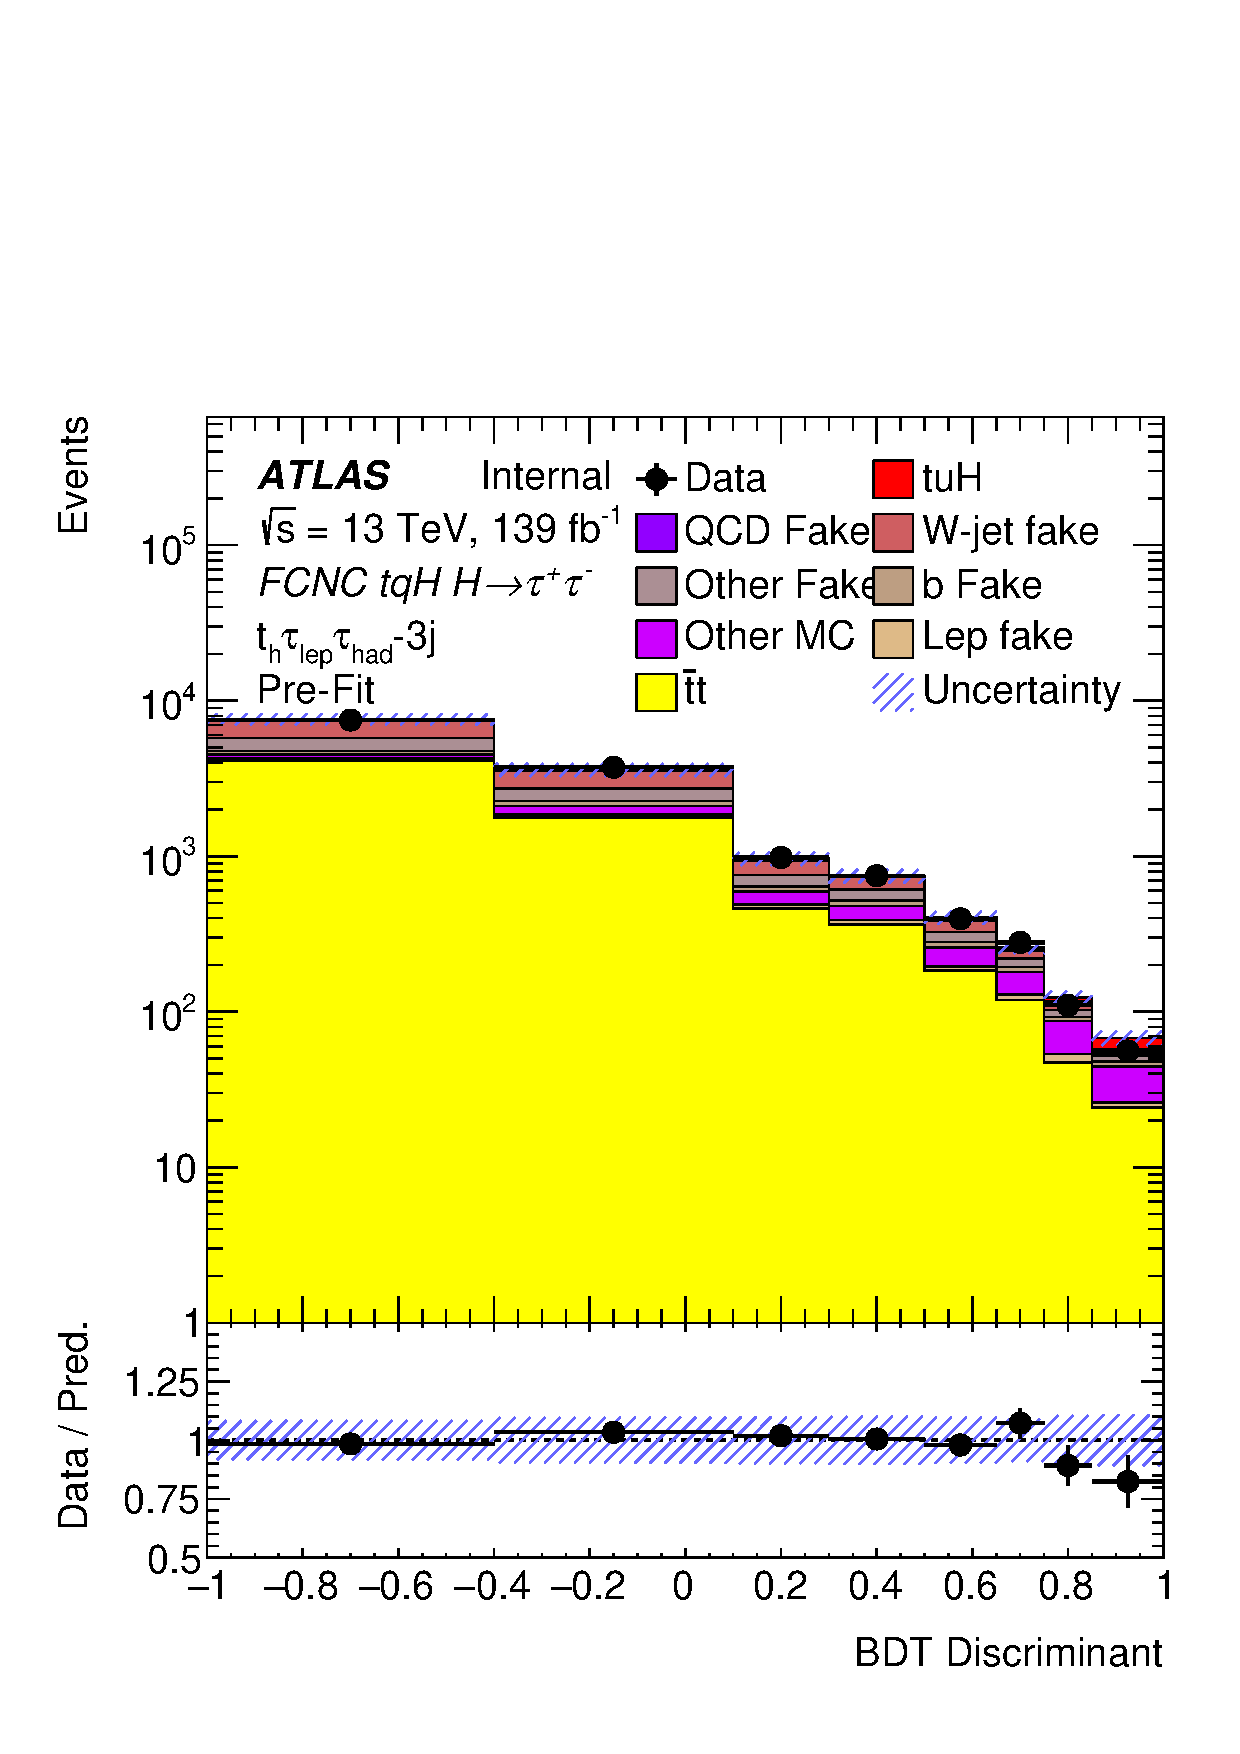
\includegraphics[width=0.45\textwidth]{/home/boyang/work/FCNCProject/FCNCAnalysis/run/trex/reg1l1tau1b3j_os_BDTG_test/Plots/reg1l1tau1b3j_os.pdf}
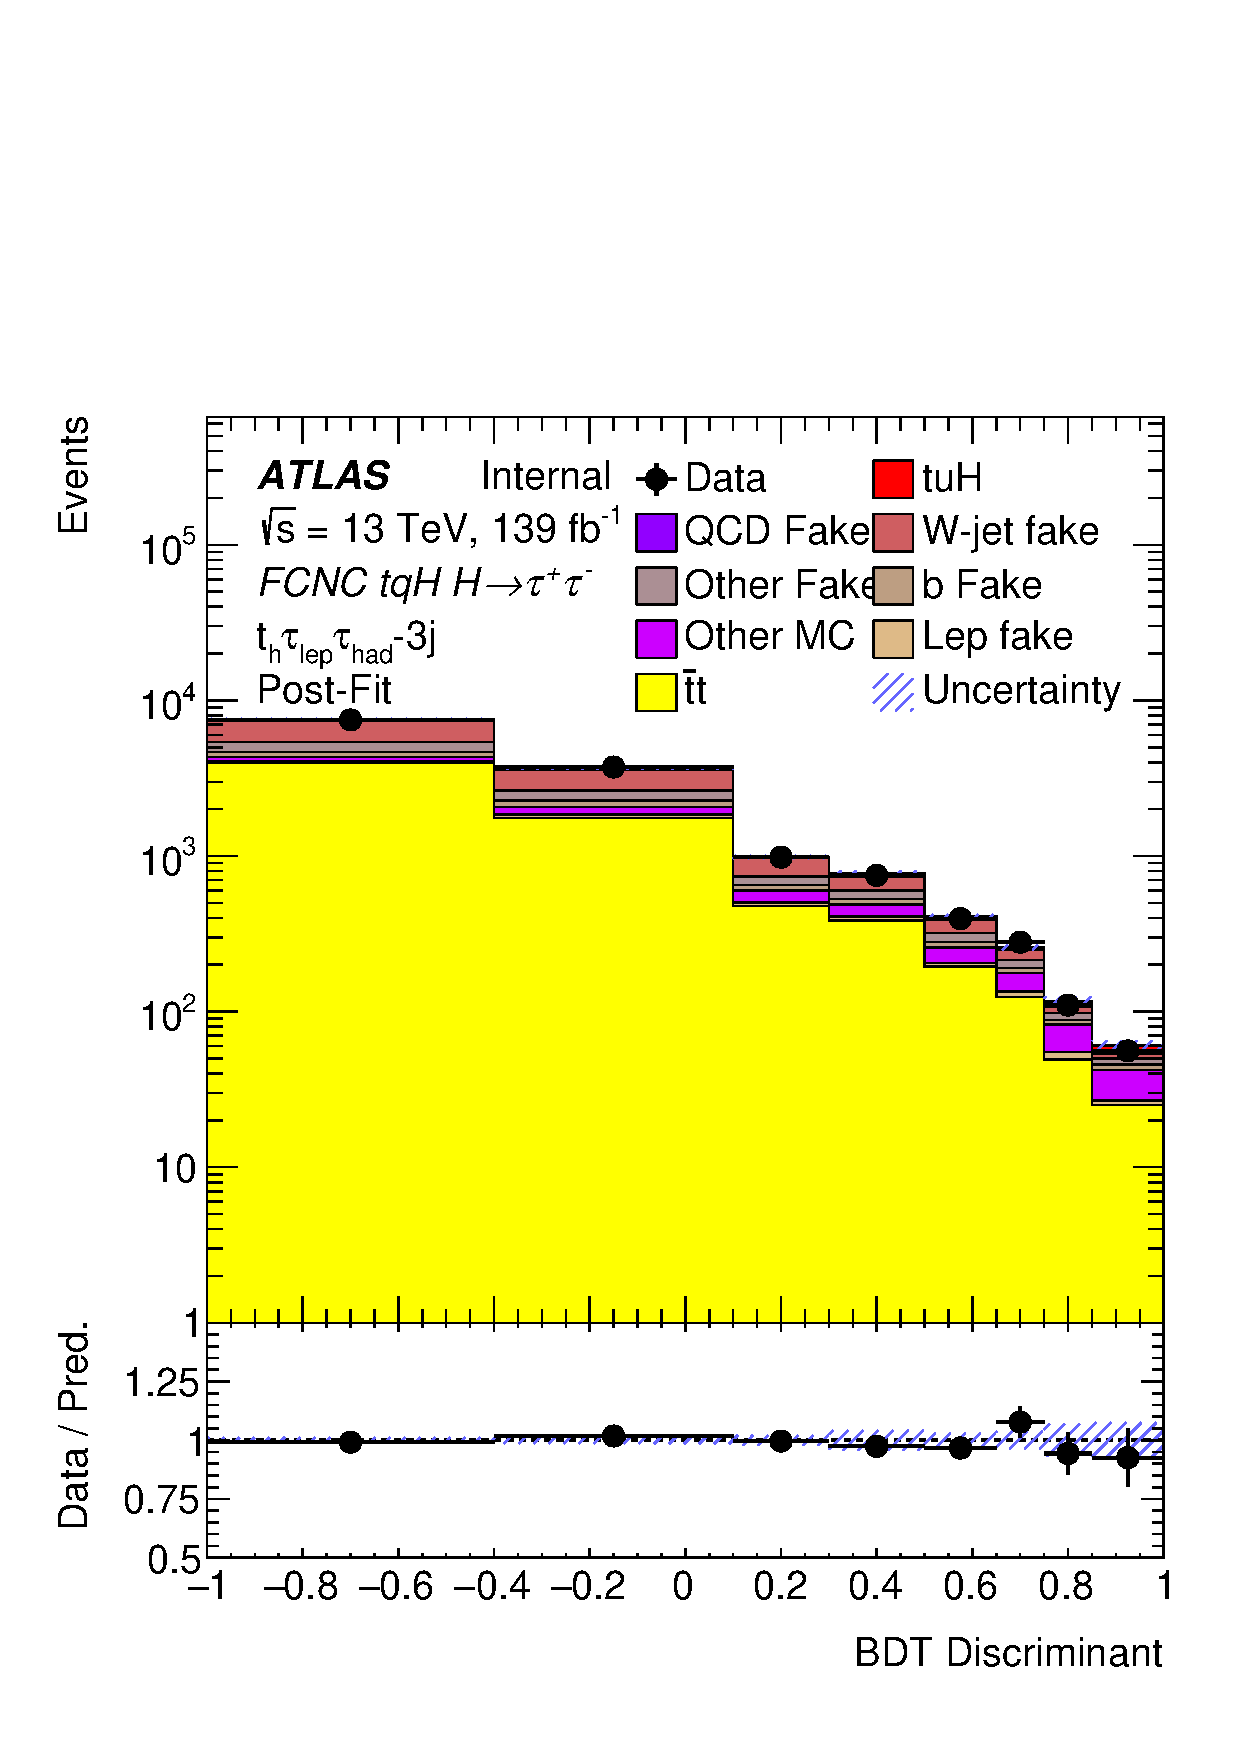
\includegraphics[width=0.45\textwidth]{/home/boyang/work/FCNCProject/FCNCAnalysis/run/trex/reg1l1tau1b3j_os_BDTG_test/Plots/reg1l1tau1b3j_os_postFit.pdf}
\label{fig:wjet_pt}
\end{figure}
\newpage
\frame{
\begin{table}
\centering
\footnotesize
\begin{tabular}{|c|c|c|c|c|} \hline
 & STH~$\tlhad$~os & TTH~$\tlhad$~os & $l\thadhad$~os & Combined\\\hline
$\bar{t}t\to bWcH$ & $2.48^{+0.98}_{-0.69}$ & $1.04^{+0.42}_{-0.29}$ & $0.31^{+0.13}_{-0.09}$ & $0.32^{+0.13}_{-0.09}$\\\hline
$cg\to tH$ & $23.16^{+9.85}_{-6.47}$ & $24.66^{+10.87}_{-6.89}$ & $3.86^{+1.67}_{-1.08}$ & $3.77^{+1.61}_{-1.05}$\\\hline
tcH merged signal & $2.25^{+0.89}_{-0.63}$ & $1.00^{+0.40}_{-0.28}$ & $0.29^{+0.12}_{-0.08}$ & $0.30^{+0.12}_{-0.08}$\\\hline
$\bar{t}t\to bWuH$ & $2.44^{+0.97}_{-0.68}$ & $0.99^{+0.40}_{-0.28}$ & $0.29^{+0.12}_{-0.08}$ & $0.30^{+0.12}_{-0.08}$\\\hline
$ug\to tH$ & $3.70^{+1.54}_{-1.03}$ & $4.30^{+1.96}_{-1.20}$ & $0.82^{+0.36}_{-0.23}$ & $0.81^{+0.34}_{-0.23}$\\\hline
tuH merged signal & $1.51^{+0.60}_{-0.42}$ & $0.80^{+0.32}_{-0.22}$ & $0.21^{+0.09}_{-0.06}$ & $0.23^{+0.09}_{-0.06}$\\\hline
\end{tabular}
\end{table}


}
\end{document}

